\section{The sample}
\label{sec:sample}

This search covers \NWindows{} spectral windows toward \NStars{} stars in
\NSystems{} systems within 40\,pc. They are drawn from \NEB{} public ALMA
execution blocks and \TotalDataTB\,TB of raw data, put through one frozen
pipeline: \StTelHours\,h of telescope time, and \LdgCensusHours\,h summed
over windows. That set is the \emph{primary census}: every
sensitivity, every expectation and every limit here is computed over it, and
so are \MtCrossACen{} of the \EvNCrossRaw{} threshold crossings this paper
reports; \LdgNCrossB{} more are coarse-channel crossings of the same census,
all of them in the one execution block that fails the data-quality criterion
of \S\ref{sec:summary}, and they are reported apart for that reason and not
because they fall outside it. The remaining \CeNTailCross{} lie in the
\emph{archival tail}: the \LdgExtTail{} execution blocks searched after the
sweep that fixed the census was closed, toward stars the census already holds,
whose \LdgExtTailWin{} windows are not tabulated window by window here and
enter no expectation. Three further sets of blocks were searched and enter no
census statistic -- the \emph{archival extension}, \LdgExtEB{} blocks and
\LdgExtWin{} windows toward \LdgExtStars{} of the same stars, run through the
frozen pipeline after the detection statistic and the line mask were fixed; a
\emph{hold-out} -- blocks set aside, by a rule fixed in advance, so that the
finished pipeline could be tested on data it had never seen;
and an out-of-sample control beyond 40\,pc -- while a rank-calibration sample
is drawn from the blocks already counted.
Table~\ref{tab:blockledger} names them in rows that sum, and
Table~\ref{tab:counts} resolves every count of windows, crossings and systems
into the set it is counted over.

\emph{Star} means one stellar component, \emph{system} a bound group
counted once however many of its components were observed, and \emph{target}
one ALMA pointing.

The census is two experiments: \NWinA{} fine-channel windows toward
\LdgClassAStars{} stars in \NSysClassA{} systems resolve a drifting carrier
-- \emph{Class~A}, and every sensitivity and exclusion quoted here refers to
them unless stated otherwise -- while the remaining \NWinB{} coarse-channel
windows support a secondary search for unresolved spectral excess with no
drift discrimination, \emph{Class~B}.

The inclusion criteria were applied by query. A star enters
if its Gaia~DR3 parallax is at least 25\,mas, measured to better than
\PlxAdqlPct{} per cent, and if its proper-motion-corrected position at the
observation epoch falls inside the quoted field of view of at least one
public execution block. Distances are direct inversions, $d=1/\varpi$, and
the star need not sit at the pointing centre. One further rule applies to the
window and not to the star: a window is kept only where the primary-beam
response at the star is at least \BmFloorResp, the offset at which the
Gaussian adopted here and the response of a blocked circular aperture
part by \BmFloorTolPct{} per cent. It removes nothing: the furthest window in
the census lies at \BmCensusWorstC\,$\lambda/D$ against a limit at
\BmFloorC\,$\lambda/D$, so the limit does not stand clear of the distribution,
and the windows it is nearest are the \BmEpsNCensusOff{} off-axis ones on
$\epsilon$~Eridani, which the survey searches.
The precision clause never binds: the worst fractional parallax
error among the stars searched is \SfPlxWorstPct{} per cent. The query returns
\NCensus{} work-list entries; the quoted field of view is optimistic, and
only \NGenuinelyCovered{} of those stars are in fact contained by a public
field, of which \NStars{} yielded a searchable window. One target has no
catalogue name -- a serendipitous field star that appears throughout as
\BkAlmaName, Gaia~DR3 \BkAlmaGaia, an \BkAlmaSpType{} dwarf at
\BkAlmaDistPc\,pc with no measured systemic velocity.

Disc, planet and colour enter as descriptive metadata only. One exclusion,
though, is a property of the catalogue and not of the sky: a Gaia~DR3
parallax needs a Gaia~DR3 source, and the brightest stars have none. Every
one of the \BsNBright{} stars in this volume brighter than \BsBrightMag{}
magnitude is absent from DR3 astrometry, and so is a steady
\BsGapFaintPct{} per cent of every magnitude bin below Hp~\BsGapMagCut,
which saturation does not explain. Together \BsNGap{} of the \BsNVol{} Hipparcos stars whose own parallaxes
meet the criteria above never reached the work list: \BsGapNBright{} of them
brighter than Hp~\BsGapMagCut{} and \BsGapNFaint{} fainter. Of these,
\BsNAlmaWord{} lie inside a public field of view -- \BsStarList{} -- and
hold \BsNWinA{} fine-channel and \BsNWinB{} coarse-channel windows. Those
windows amount to \BsRawTB\,TB of raw data in \BsNEB{} execution blocks,
none of it searched here. Sirius shows what that costs. The \BsSirNEBWord{} blocks that put
Sirius~B in this census are pointed at Sirius~A, whose catalogue position lies
within \BsSirSepA{} arcsec of the delivered phase centre, while the companion
was read \BsSirOffLo--\BsSirOffHi{} arcsec off axis in the same
\BsSirNWin{} windows. Each block's continuum map holds the primary at
\BsSirSnrLo--\BsSirSnrHi{} times its own noise, with spectral index
\BsSirAlpha, and nothing at the companion. The primary is displaced
\BsSirCenLo--\BsSirCenHi{} arcsec from its catalogue position by its own
orbit, where the orbit of \citet{bond2017} predicts \OmSirPredArcsec{}
arcsec, in the measured direction to within the block-to-block scatter of the
centroid. So the brightest star in the sky was measured three times by this
survey and reported at neither position. \BsNoFineList{} carry no fine-channel
window at all, so they would add a constraint on unresolved excess rather
than a carrier limit; the \BsNFineWord{} that do are \BsFineList,
\BsNFineATypeWord{} of them A~stars with bright debris discs. A search of
this volume should admit these stars on Hipparcos astrometry where Gaia has
none.

Two removals act on windows rather than on stars, and account for the whole
difference between the
\LqNExport{} rows the extraction wrote and the \NWindows{} retained:
\NDup{} repeated rows of one window and
\NDefect{} failing a quality cut that is physical rather than chosen; the
primary-beam limit above removes none.
Since $\sigma\sqrt{t_{\rm on}\Delta\nu_{\rm ch}}$ is set by system
temperature and collecting area, a window more than \LqDefectCut{} times
below the sample median in it is not measuring the sky; those removed lie
$\LqDefectFacLo$--$\LqDefectFacHi$ times below and the nearest retained
\LqKeptFac{} times, so the level is not a tuned one. No integration-time cut
was applied; the shortest window retained carries \LqOnsrcMin\,s on source.

\subsection{The archival selection}
\label{sec:bias}

This sample was not designed: it is whatever previous ALMA programmes
happened to observe among the stars Gaia~DR3 catalogues, and
\PctDiscProposal{} per cent of the stars searched were targeted under a
debris-disc or planet-formation proposal. Table~\ref{tab:selfunc} measures
the bias against a volume-limited reference census of which the searched
stars are a subset, classifying both columns by one rule so that every ratio
below is like against like. Both columns are Gaia-defined, so neither
contains the bright stars above and the ratios are internally consistent
without them.

The dominant selection effect is distance. Stars within 5\,pc are
over-represented by a factor \SfTopRatio, and the enhancement falls
monotonically with distance to a factor of two \emph{under}-representation
beyond 30\,pc. Colour comes second: A~stars are over-represented by about
\SfARatio{} and F and G stars by factors of three, because those are the
stars with bright debris discs. For the A~stars that factor is a floor,
because the catalogue requirement is itself colour-selective: it removes
\BsNEarly{} of the \BsNEarlyVol{} stars in the volume as blue as an A~star,
\BsEarlyRatio{} times its rate among all the others. M~dwarfs are depleted
--
\SfMSearched{} of the \SfNStar{} searched stars are M~dwarfs, a factor
\SfMRatio{} of their share of the reference census, and only
\SfMClassAStars{} of them carry the fine-channel coverage that can resolve a
drifting carrier at all. Coverage is also concentrated:
\ConcThreeWin{} of the \NWindows{} windows come from \ConcThreeSys{}
systems. No statement in this paper is therefore an occurrence rate for the
solar neighbourhood, and the selection acts hardest on
exactly the targets a designed search would pick: of the \CsIntNRow{} sample
systems within 15\,pc with a confirmed planet, \CsIntNoClassA{} carry no
Class~A coverage and so no drift-resolving limit.

%% GENERATED by selfunc_v411.py -- do not hand-edit.
\begin{table}
\centering
\scriptsize
\setlength{\tabcolsep}{4pt}
\caption{Selection function of the searched sample against a volume-limited reference census. Both columns are the same Gaia~DR3 selection -- $\varpi>0$, $\sigma_\varpi/\varpi\le0.1$ and $1/\varpi\le40$\,pc, 17\,566 objects -- of which the 90 searched stars are rows. The survey's own criterion is the looser $\sigma_\varpi/\varpi\le0.2$ of \S\ref{sec:sample}, at which this census holds the same 17\,566 objects, so the two cuts are one selection and not two; and both are classified by one rule, in which BP$-$RP colour sets the class and the absolute G magnitude separates the degenerates that colour alone would place among the A~stars. The rule reaches 17\,278 census objects and 88 of the 90 searched stars, the rest carrying no Gaia BP or RP photometry. ``Ratio'' is the searched column fraction over the census column fraction; $>1$ is over-representation. The strongest selection effect here is distance, not colour.}
\label{tab:selfunc}
\begin{tabular}{@{}lrrr@{}}
\toprule
Property & Census & Searched & Ratio \\
\midrule
\multicolumn{4}{@{}l}{Distance} \\
\quad $d\le5$\,pc & 48 (0.3\%) & 13 (14.4\%) & 52.9 \\
\quad 5--10\,pc & 240 (1.4\%) & 13 (14.4\%) & 10.6 \\
\quad 10--20\,pc & 2069 (11.8\%) & 18 (20.0\%) & 1.7 \\
\quad 20--30\,pc & 5391 (30.7\%) & 19 (21.1\%) & 0.7 \\
\quad 30--40\,pc & 9818 (55.9\%) & 27 (30.0\%) & 0.5 \\
\midrule
\multicolumn{4}{@{}l}{Colour class$^{a}$} \\
\quad A & 61 (0.4\%) & 5 (6.2\%) & 17.2 \\
\quad F & 473 (2.8\%) & 8 (10.0\%) & 3.6 \\
\quad G & 978 (5.8\%) & 15 (18.8\%) & 3.2 \\
\quad K & 2221 (13.2\%) & 11 (13.8\%) & 1.0 \\
\quad M & 13\,082 (77.8\%) & 41 (51.2\%) & 0.7 \\
\midrule
\multicolumn{4}{@{}l}{Other axes} \\
\quad Confirmed planet hosts$^{b}$ & 26 (15.5\%) & 24 (26.7\%) & 1.7 \\
\quad White dwarfs$^{a}$ & 463 (2.7\%) & 8 (8.9\%) & 3.3 \\
\quad Searched stars / systems & -- & 90 / 83 & -- \\
\bottomrule
\end{tabular}

\smallskip
{\footnotesize $^{a}$Colour bins, not MK types. The boundaries are the colours at which the census's own temperature--colour relation crosses 7500, 6000, 5300 and 3900\,K: BP$-$RP $<0.36$ for A, 0.36--0.72 for F, 0.72--0.95 for G, 0.95--1.77 for K and $>1.77$ for M. Over the 8594 census objects that also carry a Gaia temperature the two classifications agree for 98 per cent, and every disagreement is between neighbouring bins. A star is counted as degenerate when it lies more than 4\,mag below the main sequence measured from the census itself: the two sequences are separated by 5 to 8\,mag here, so moving the cut by a magnitude either way changes the count by under 3 per cent. The five classes are normalised over the 80 non-degenerate searched stars and the 16\,815 non-degenerate census objects.\\ $^{b}$Both columns are the same positional join, of the 168-entry ALMA-covered work list and of its searched subset, to the NASA Exoplanet Archive \texttt{pscomppars} table accessed 2026 October 4. The 24 searched hosts carry 51 confirmed planets, 22 of the 24 surviving the deuterium-burning mass limit; the Gaia census carries no planet information, so the census column in this row is the work list and not the 17\,566-object Gaia census.}
\end{table}


%% fig:funnel DELETED: it drew the three counts the sentence above it
%% already carries, so it joined the prose instead of replacing it.  The
%% artwork is online material (figures_diagnostic/selection_funnel.pdf).

\subsection{Frequency coverage and archival scope}
\label{sec:coverage}

The Class~A experiment covers $\Delta\nu_A=\DnuA$\,GHz of unique sky
frequency, and that coverage is sparse: \DomAIslands{} disjoint islands
between \DomAFreqLo{} and \DomAFreqHi\,GHz rather than a band, so those
endpoints bound where observations exist and not what was covered. With the
coarse-channel windows the archival coverage is \DnuAB\,GHz in
\UnionIntervals{} intervals, of which \SearchedUnionGHz\,GHz survives the
molecular-line mask of \S\ref{sec:method}. Fig.~\ref{fig:waterfall} shows the
distribution: a transmitter between the islands was never observable here,
whatever its power.

The archive is not exhausted either. \LdgExtScope{} further blocks lie inside
the same query and were unprocessed when the census was frozen, of which
\LdgExtSearched{} carry a calibration and are searched. \LdgExtEB{} of those
are reported here as repeat epochs. The remaining \BkExtNotReported{} are
accounted for in Table~\ref{tab:blockledger} row by row: \QbkNTail{}
archival-tail blocks, whose \QbkNTailCross{} threshold crossings enter no
expectation; \QbkNEps{} $\epsilon$~Eri blocks, which contribute only the
limits of Appendix~\ref{app:conventions}; and \QbkNNoWin{} from which no
window reached the export. The largest single gap is the \FateNoCal{} blocks whose raw visibilities
the archive holds but never pipeline-calibrated, \FateNoCalGB\,GB in all; no
effort of ours would close that.

\begin{figure*}
\centering
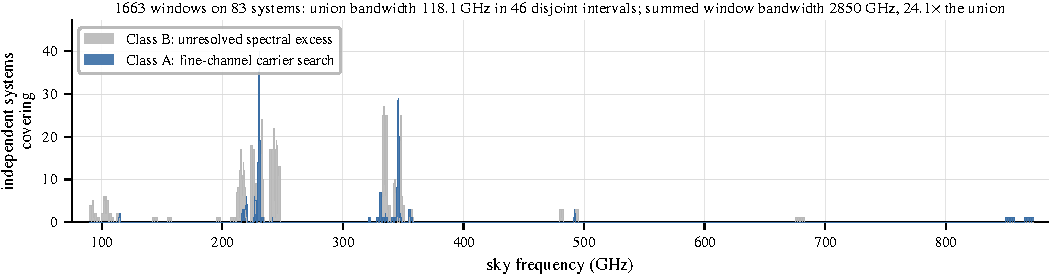
\includegraphics[width=0.99\textwidth]{figures/coverage_waterfall.pdf}
\caption{Where this survey searched: the number of independent systems
covering each sky frequency, drawn separately for the two experiments --
blue the fine-channel carrier search (Class~A), light grey the coarse-channel
spectral-excess search (Class~B). Each curve steps at the searched window
edges themselves rather than on a grid, so an interval narrower than a plotted
pixel still appears. The summed window bandwidth is $\GrossOverUnion\times$
the union, so the union measures frequency coverage and the summed bandwidth
search effort.}
\label{fig:waterfall}
\end{figure*}

%% Floats that belong elsewhere: tab:blockledger is in Appendix A (its
%% headline rows are in the prose above, so the cross-reference is not a
%% pointer with no numbers beside it); tab:interesting is neither typeset nor
%% distributed -- r15-deposit, 2026-10-08: there is no deposit, so if its rows
%% are wanted by a reader they have to be printed; tab:searchspace is deleted, nothing having cited
%% it, and its counts, unions, channel widths and drift range are all
%% elsewhere in the paper.
%% Carried forward to the numbers owner: tab_interesting.tex is still
%% generated but is not in make_all.sh, and its planet column should read the
%% dated NASA Exoplanet Archive extract selfunc_v411.py uses so that one
%% definition of "confirmed planet" serves both tables.  Two display defects
%% belong in star_alias.designation: Barnard's Star prints as a SIMBAD
%% identifier with the "NAME" prefix stripped, and BD+05 1668 would read
%% better with its GJ alias beside it.
